\documentclass[a4paper,12pt]{article}
\usepackage[T2A]{fontenc}
\usepackage[utf8]{inputenc}
\usepackage[russian]{babel}
\usepackage{amsmath, amssymb}
\usepackage{setspace}
\usepackage[left=2cm, right=2cm, top=2cm, bottom=2cm]{geometry}
\usepackage{graphicx}
\usepackage{listings}
\usepackage{xcolor} % Для подсветки
\usepackage{float} 

\begin{document}
\section*{Задание 3}
$$\left\{
\begin{aligned}
  u_{xx} &= f(x), \quad &x \in (0,1) \\
  u|_{t=0} &= 2, \\
  u|_{t=0} &= 0, \\
  u_x|_{x=0} &= t, \\
  u_x|_{x = l} = -1
\end{aligned}
\right\}$$

$$u = v + \omega$$

$$\omega = \frac{-t-1}{l}x^2 + tx$$
$$
\begin{cases}
v_{tt} - v_{xx} = t^2 - \frac{t+1}{l} - x \\
v|_{t=0} = 2 + \frac{x^2}{l}, \\
v_t|_{t=0} = 0, \\
v_x|_{x=0} = 0, \\
v_x|_{x=l} = 0
\end{cases}
$$

Будем искать решение в виде: $v = TX$

$$T'' X = a^2 T X'' $$
$$\frac{T''}{a^2 T} = \frac{X''}{X} = -\lambda$$

$$X_k = C_1 \cos\sqrt{\lambda}x + C_2 \sin\sqrt{\lambda}x$$

$$X_k'|_{x = 0} = 0 \Rightarrow C_2 = 0$$

$$X_k'|_{x = \ell} = C_1 \sqrt{\lambda} \sin(\sqrt{\lambda} \ell) = 0 \Rightarrow \sin(\sqrt{\lambda} \ell) = 0 \Rightarrow \sqrt{\lambda_k} = \frac{\pi k}{\ell}$$

$$X_k = \cos\left( \frac{\pi k}{\ell} x \right)$$

$$P = \sum_{k=1}^{\infty} T_k \cos\left( \frac{\pi k}{\ell} x \right)$$

\textbf{Подставим:}
$$\sum_{k=1}^{\infty} \left( T_k'' + \left( \frac{\pi k}{\ell} \right)^2 T_k \right) \cos\left( \frac{\pi k}{\ell} x \right) = t^2 - \frac{t+1}{l} - x$$

\textbf{Разложим в ряд Фурье:}
$$t^2 - \frac{t+1}{l} - x = \sum_{k=1}^{\infty} T_k X_k = \sum_{k=1}^{\infty} \frac{2(1 - \cos k \ell)}{\pi k} \cos\left( \frac{\pi k}{\ell} x \right)$$

\textbf{Имеем:}
$$T_k'' + \left( \frac{\pi k}{\ell} \right)^2 T_k = \frac{2(1 - \cos(k \ell))}{\pi k}$$

\textbf{Разложим $\phi = 2 + \dfrac{x^2}{l}$ в ряд Фурье}

$$\phi = \sum_{k=1}^{\infty} \frac{2l\cos(\pi k)}{(\pi k)^2} \cos\left( \frac{\pi k}{l} x \right)$$



\textbf{Подставим в начальные условия:}
$$\sum_{k=1}^{\infty}T_k cos(\frac{\pi k}{l}x)|_{t=0} = \sum_{k=1}^{\infty}\frac{2lcos(\pi k)}{(\pi k)^2}cos(\frac{\pi k}{l}x)$$
\textbf{Отсюда имеем:}
$$T_k|_{t=0} = \frac{2l cos(\pi k)}{(\pi k)^2}$$
$$
\begin{cases}
    T_k'' + \frac{\pi k}{l}T_k = \frac{2(1 - \cos(k \ell))}{\pi k} \\
    T_k|_{t=0} = \frac{2l cos(\pi k)}{(\pi k)^2} \\
    T_k'|_{t=0} = 0
\end{cases}
$$
$$T_k = A_k cos(\frac{\pi kt}{l}) + B_k sin(\frac{\pi kt}{l})$$
$$T_k |_{t=0} = \frac{2l cos(\pi k)}{(\pi k)^2} \Rightarrow A_k = \frac{2l cos(\pi k)}{(\pi k)^2}$$
$$T_k' |_{t=0} = \frac{\pi k}{l}B_k = 0 \Rightarrow B_k = 0$$
\textbf{Таким образом:}
$$T_k = \frac{2l cos(\pi k)}{(\pi k)^2}cos(\frac{\pi k t}{l})$$
$$v = \sum_{k=1}^{\infty}X_k T_k = \sum_{k=1}^{\infty} \frac{2l cos(\pi k)}{(\pi k)^2}cos(\frac{\pi k t}{l})cos(\frac{\pi k x}{l})$$
$$u = \sum_{k=1}^{\infty}X_k T_k = \sum_{k=1}^{\infty} \frac{2l cos(\pi k)}{(\pi k)^2}cos(\frac{\pi k t}{l})cos(\frac{\pi k x}{l}) - \frac{t+1}{l}x^2 + tx$$

\section*{Визуализация 1}
$$u(x,t) = \sum_{k=1}^\infty \left( \frac{16 g l^2}{a^2 (\pi + 2 x k)^3} \sin \frac{a \sqrt{(\pi + 2 x k)^2}}{2 l} t \right) \sin \frac{\pi - 2 k}{2 l} x$$
\textbf{Ниже приведен код на языке Python, который изображает график данной функции}
\begin{lstlisting}
import numpy as np
import matplotlib.pyplot as plt
from mpl_toolkits.mplot3d import Axes3D

g = 9.8
l = 1
a = 1

x = np.linspace(0, 2 * l, 200)
t = np.linspace(0, 5, 200)
X, T = np.meshgrid(x, t)

U = np.zeros_like(X)
for k in range(1, 101):
    coef = (16 * g * l**2) / (a**2 * (np.pi + 2*k)**3)
    omega_k = a * (np.pi + 2*k) / (2 * l)
    U += coef * np.sin(omega_k * T) * np.sin((np.pi - 2*k) * X / (2 * l))

fig = plt.figure(figsize=(12, 6))
ax = fig.add_subplot(111, projection='3d')
ax.plot_surface(X, T, U, cmap='viridis')

ax.set_title('u(x, t)')
ax.set_xlabel('x')
ax.set_ylabel('t')
ax.set_zlabel('u(x, t)')

plt.savefig("graph1.png", dpi=300)
plt.show()
\end{lstlisting}

\begin{figure}[H]
    \centering
    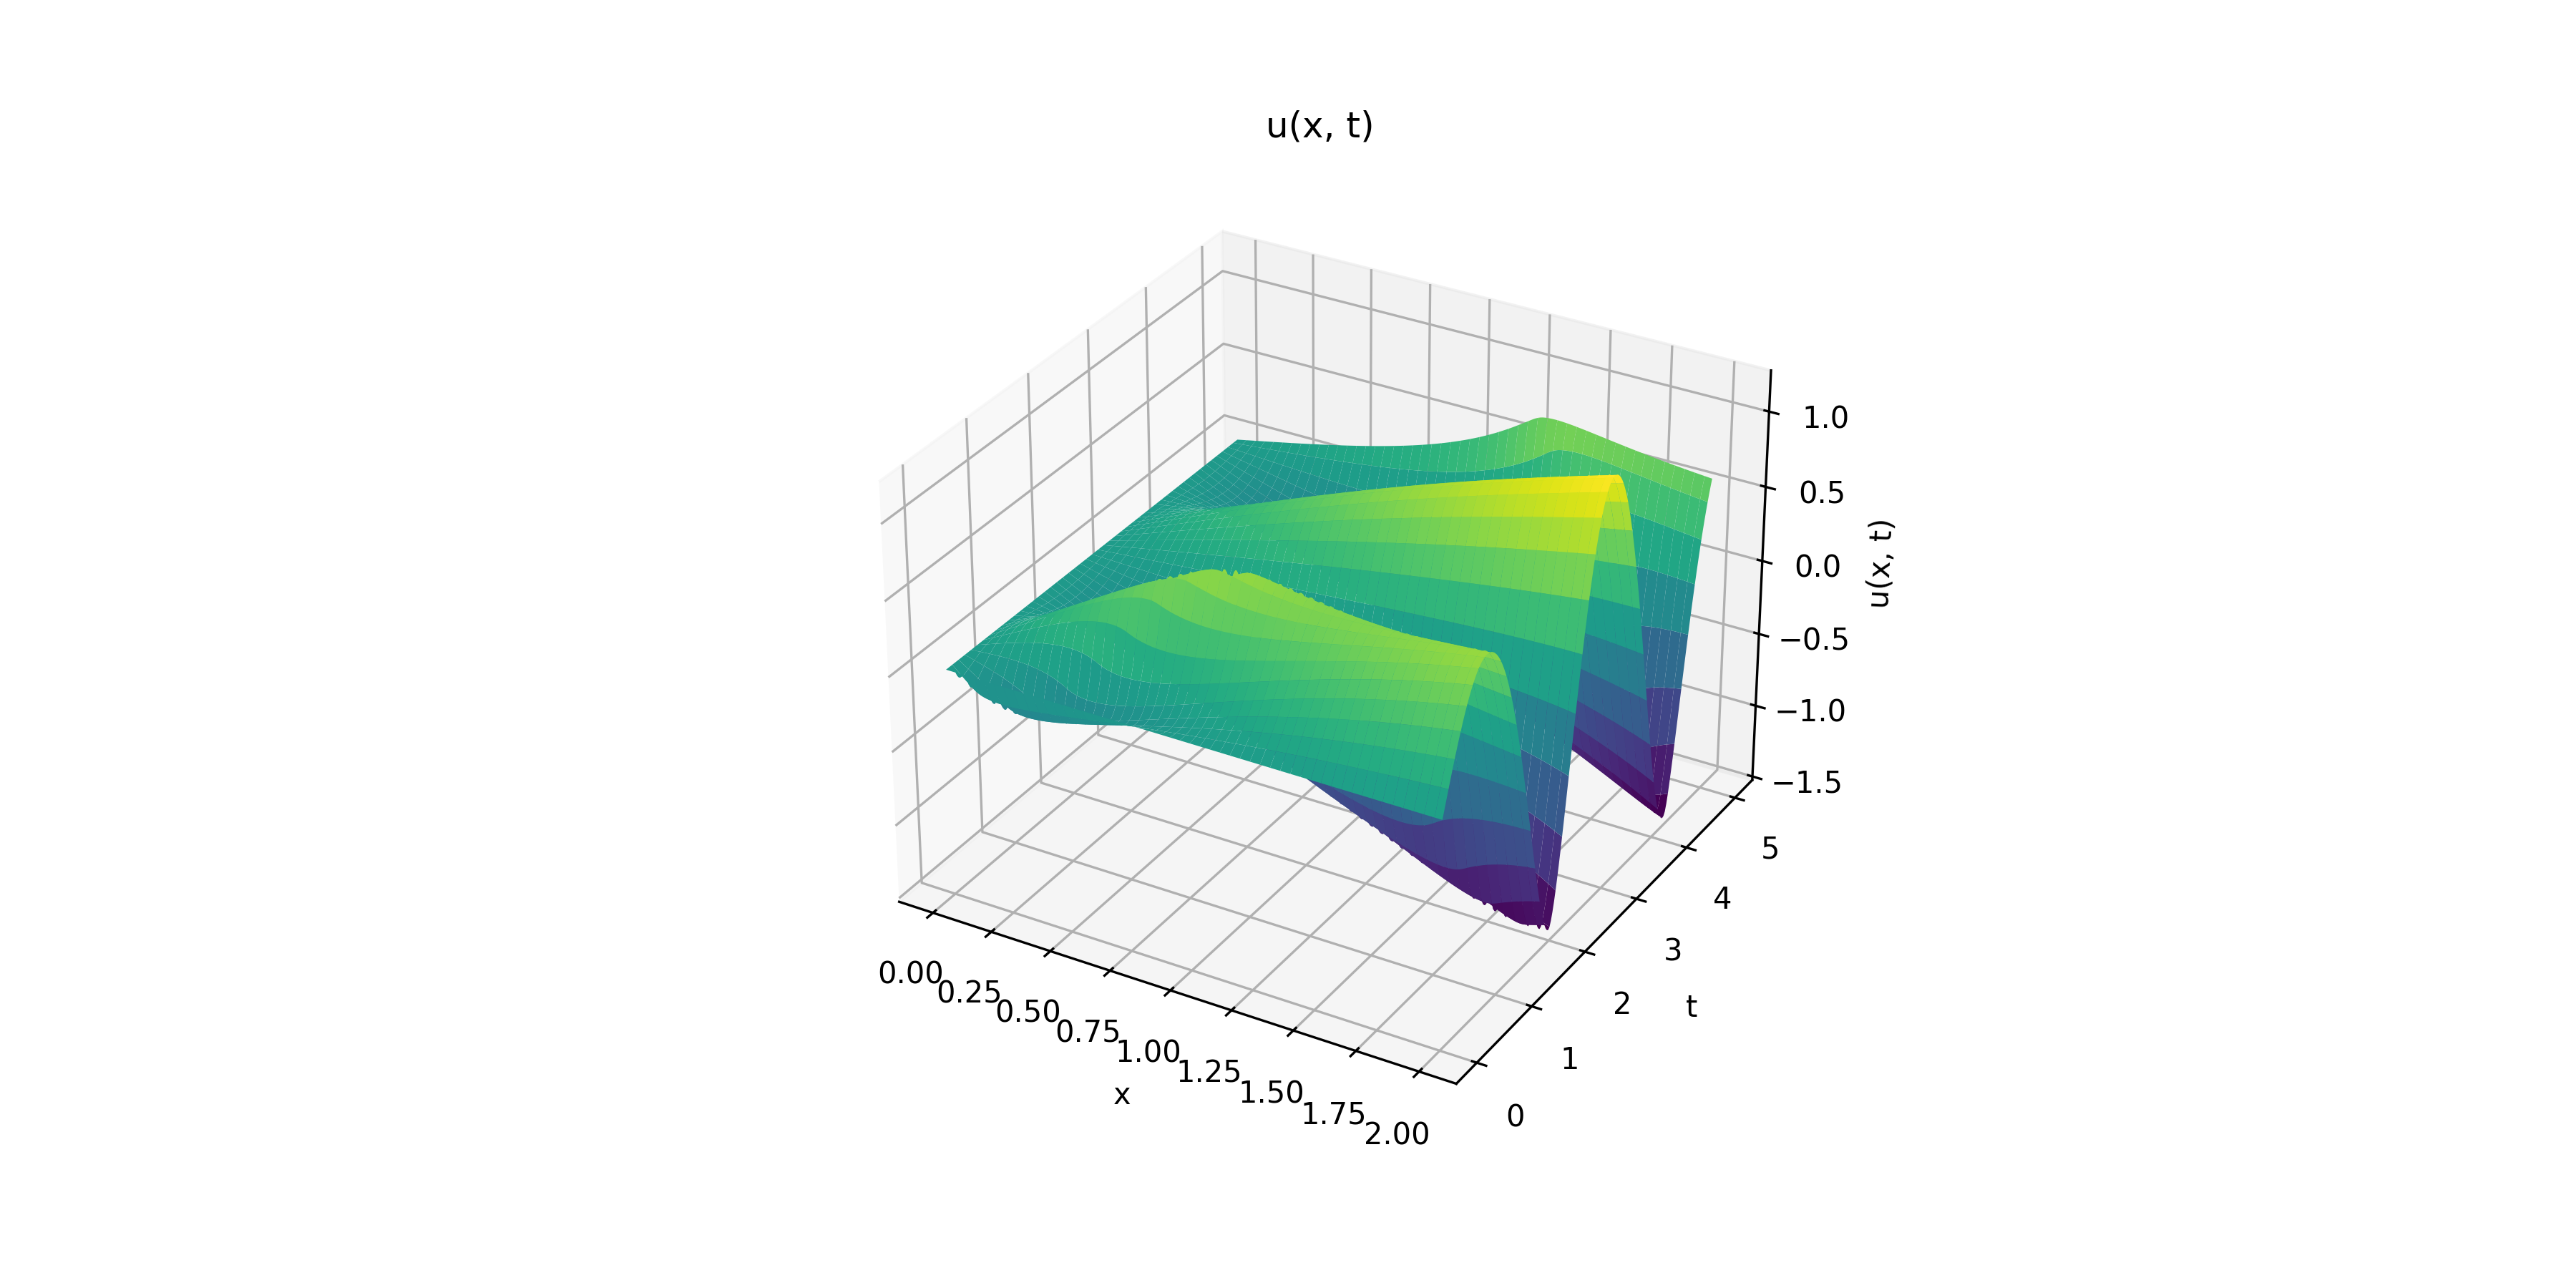
\includegraphics[width=0.8\textwidth]{../../graph1.png}
    \caption{График функции $u(x,t)$, построенный по приближённой сумме ряда}

\end{figure}

\textbf{Код проверки}
\begin{lstlisting}
    
a = 1; 
l = 1; 
g = 9.8; 
v = 1; 
solution = DSolve[{
    D[u[x, t], {t, 2}] == a^2*D[u[x, t], {x, 2}] + g,
    u[0, t] == 0,
    u[l, t] == 0,
    u[x, 0] == 0,
    Derivative[0, 1][u][x, 0] == v
}, u[x, t], {x, t}]

simplifiedSolution = FullSimplify[u[x, t] /. solution[[1]]]
\end{lstlisting}
\textbf{Результат проверки}
\begin{lstlisting}
    u[x_, t_] := Sum[
    (16 g l^2)/(a^2 (\pi + 2 x k)^3) * 
    Sin[(a Sqrt[(\pi + 2 x k)^2]/(2 l) t] * 
    Sin[(\pi - 2 k)/(2 l) x],
    {k, 1, \infty}
];
\end{lstlisting}

\section*{Визуализация 2}
$$u(x,t) = \left(1 - \frac{lt}{2at} + \left(\frac{l}{2at}\right)^2 \sin \frac{2a\pi t}{e} \cos \frac{a\pi t}{e} - \left(\frac{l}{at}\right)^2 \cdot \frac{1}{2} \sin^3 \frac{a\pi t}{e} \right) \cdot \sin \frac{\pi x}{e}$$
$$ + \sum_{k=1}^{\infty} \left( -2 \cdot \frac{\cos kl}{k \cos kl} \cos \frac{a k \pi t}{e} + \sin \frac{kl}{e} x \right)$$
\textbf{Ниже приведен код на языке Python, который изображает график данной функции}
\begin{lstlisting}
  import numpy as np
import matplotlib.pyplot as plt

from mpl_toolkits.mplot3d import Axes3D

a = 1
l = 1
e = 1
N = 100  
x = np.linspace(0, e, 200)
t = np.linspace(0.1, 5, 200)
X, T = np.meshgrid(x, t)

term1 = (1 - l / (2 * a) + ((l / (2 * a * T))**2) * np.sin(2 * a * np.pi * T / e) * np.cos(a * np.pi * T / e) -
         0.5 * (l / (a * T))**2 * np.sin(a * np.pi * T / e)**3) * np.sin(np.pi * X / e)

term2 = np.zeros_like(X)

for k in range(1, N + 1):
    denom = k * np.cos(k * l)
    if np.any(np.isclose(denom, 0)):
        continue
    term2 += (-2 * np.cos(k * l) / denom) * np.cos(a * k * np.pi * T / e) + np.sin((k * l / e) * X)

U = term1 + term2

fig = plt.figure(figsize=(12, 6))
ax = fig.add_subplot(111, projection='3d')
ax.plot_surface(X, T, U, cmap='plasma')

ax.set_title("u(x, t)")
ax.set_xlabel("x")
ax.set_ylabel("t")
ax.set_zlabel("u(x, t)")

plt.tight_layout()
plt.savefig("graph2.png", dpi=300)
plt.show()

\end{lstlisting}
\begin{figure}[H]
    \centering
    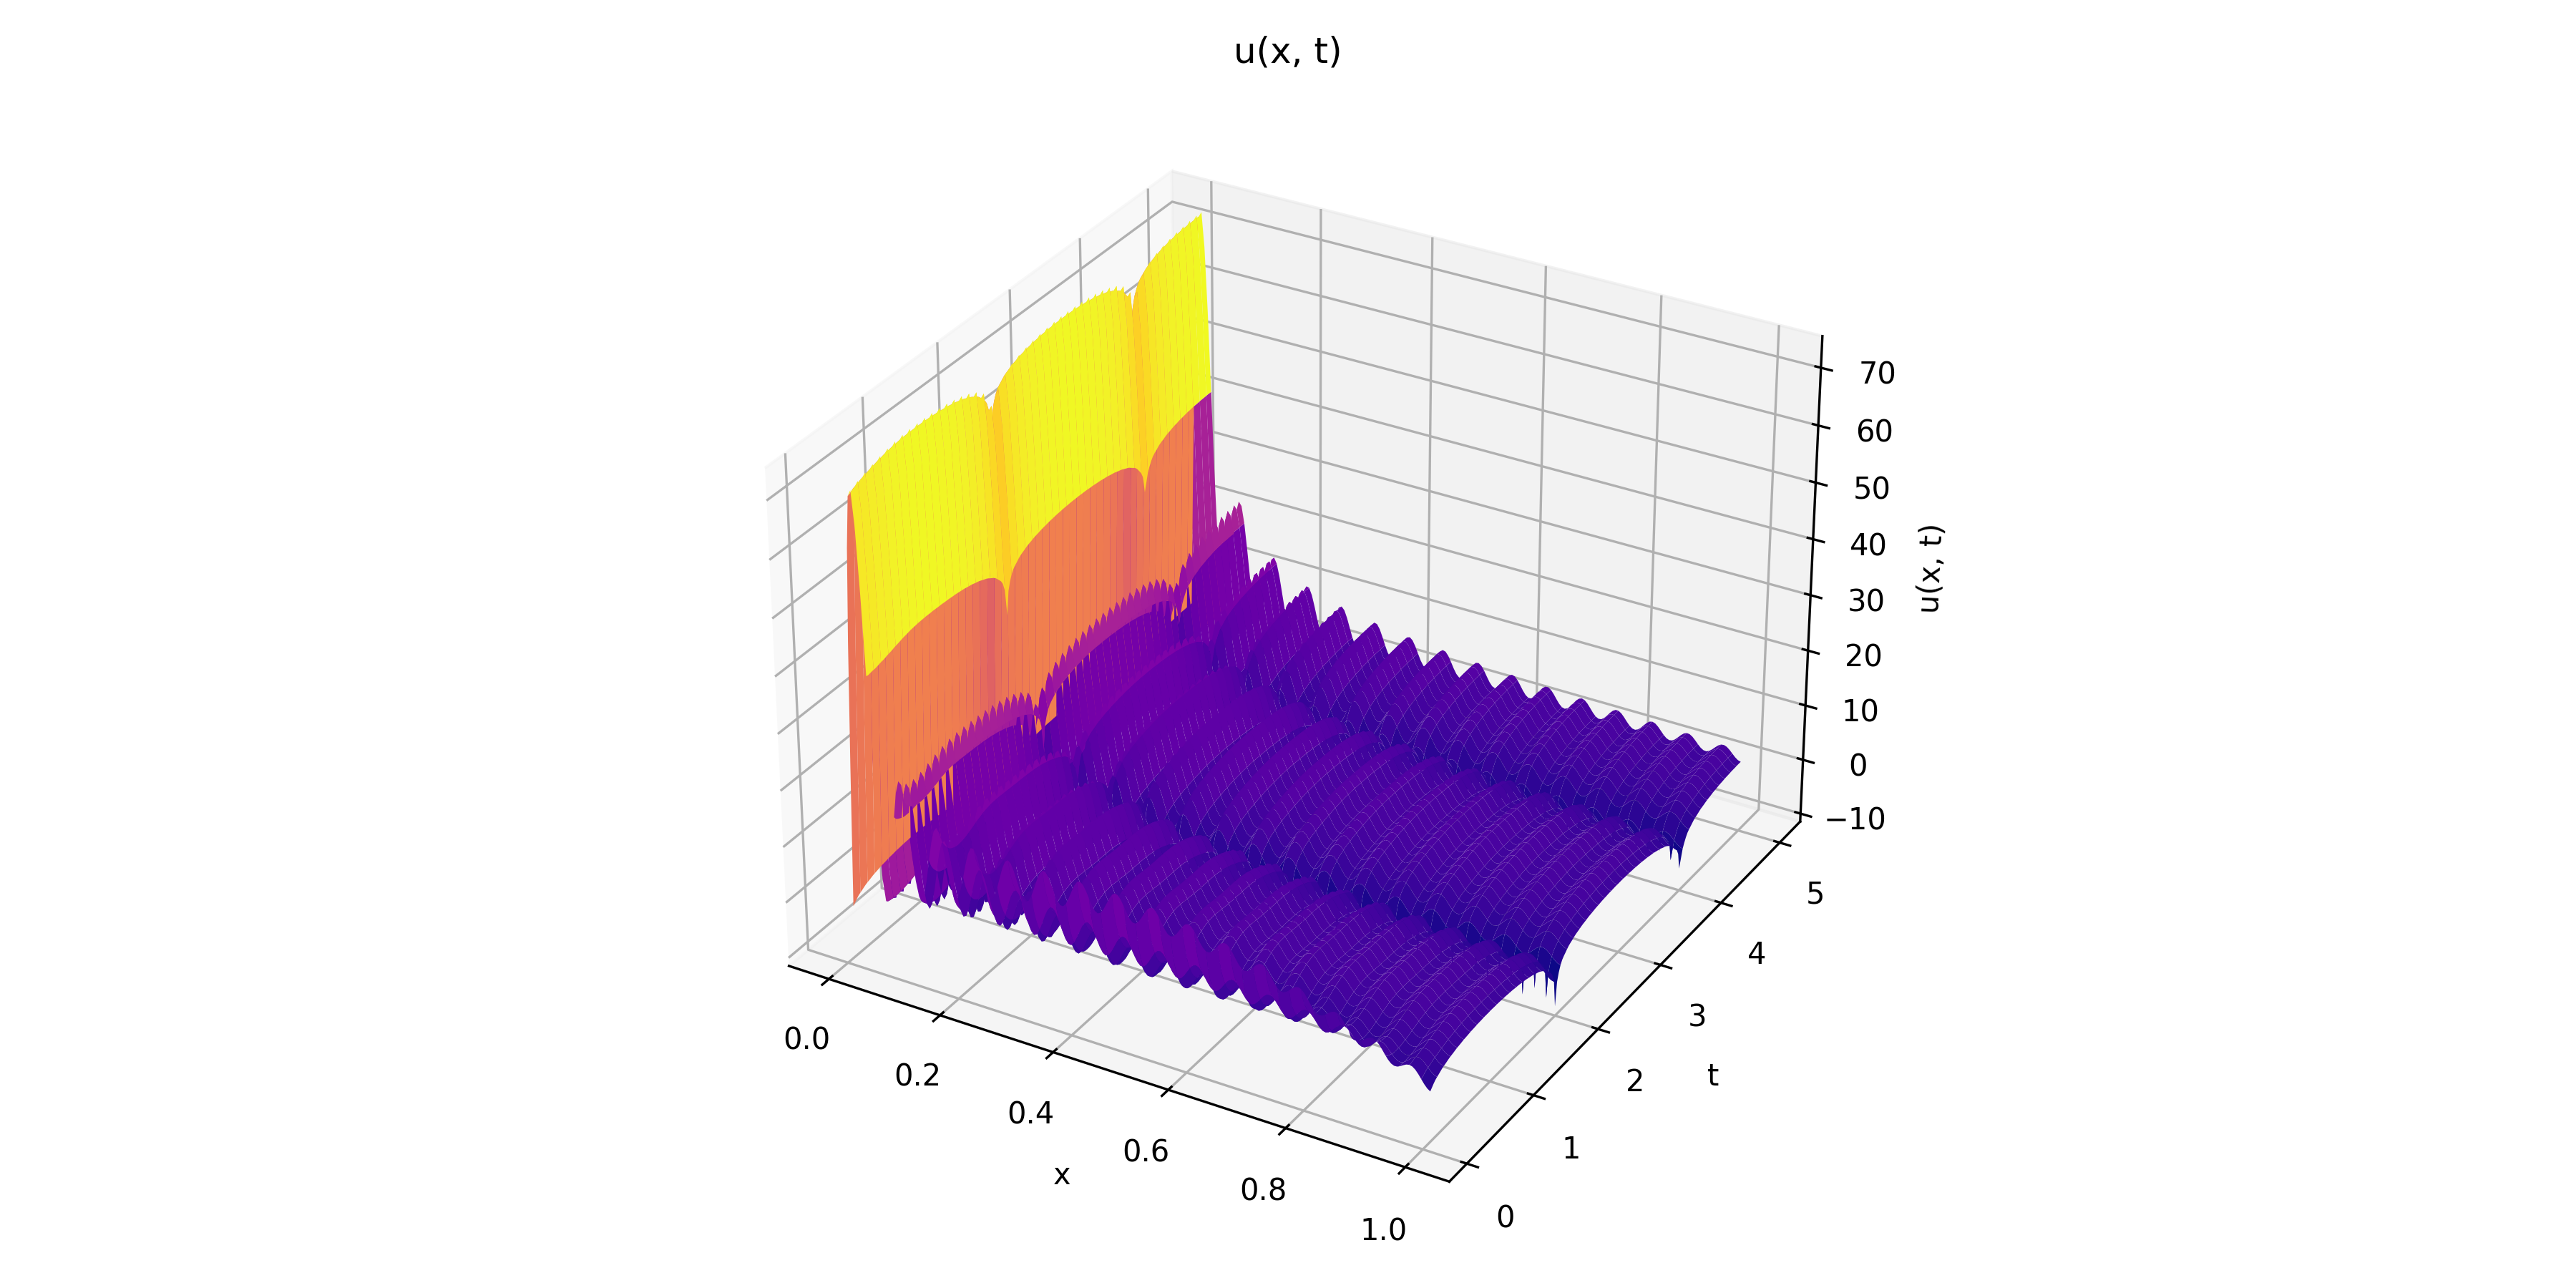
\includegraphics[width=0.8\textwidth]{../../graph2.png}
    \caption{График функции $u(x,t)$, построенный по приближённой сумме ряда}
\end{figure}

\textbf{Код проверки:}
\begin{lstlisting}
a = 1;  
l = Pi; 

solution = DSolve[{
    D[u[x, t], {t, 2}] == a^2*D[u[x, t], {x, 2}] + Sin[Pi*x/l]*Sin[Pi*t/l],
    u[0, t] == 0,
    u[l, t] == 0,
    u[x, 0] == 2*x,
    Derivative[0, 1][u][x, 0] == 0
}, u[x, t], {x, t}]

simplifiedSolution = FullSimplify[u[x, t] /. solution[[1]]]
\end{lstlisting}

\textbf{Результат проверки:}
\begin{lstlisting}
    u[x_, t_] := (1 - (l*t)/(2*a*t) + (l/(2*a*t))^2*Sin[(2*a*Pi*t)/E]*Cos[(a*Pi*t)/E] - 
             (l/(a*t))^2*(1/2)*Sin[(a*Pi*t)/E]^3)*Sin[(Pi*x)/E] + 
             Sum[(-2*(Cos[k*l]/(k*Cos[k*l]))*Cos[(a*k*Pi*t)/E] + Sin[(k*l*x)/E], {k, 1, Infinity}]

TraditionalForm[u[x, t]]
\end{lstlisting}

\section*{Визуализация 3}
$$u = \sum_{k=1}^{\infty}X_k T_k = \sum_{k=1}^{\infty} \frac{2l cos(\pi k)}{(\pi k)^2}cos(\frac{\pi k t}{l})cos(\frac{\pi k x}{l}) - \frac{t+1}{l}x^2 + tx$$
\textbf{Ниже приведен код на языке Python, который изображает график данной функции}
\begin{lstlisting}
  import numpy as np
import matplotlib.pyplot as plt
from mpl_toolkits.mplot3d import Axes3D

l = 1
N = 100 
x = np.linspace(0, l, 200)
t = np.linspace(0, 5, 200)
X, T = np.meshgrid(x, t)

U = np.zeros_like(X)

for k in range(1, N + 1):
    coef = (2 * l * np.cos(np.pi * k)) / ((np.pi * k)**2)
    U += coef * np.cos(np.pi * k * T / l) * np.cos(np.pi * k * X / l)

U += -((T + 1) / l) * X**2 + T * X

fig = plt.figure(figsize=(12, 6))
ax = fig.add_subplot(111, projection='3d')
ax.plot_surface(X, T, U, cmap='inferno')

ax.set_title("u(x, t)")
ax.set_xlabel("x")
ax.set_ylabel("t")
ax.set_zlabel("u(x, t)")

plt.tight_layout()
plt.savefig("graph3.png", dpi=300)
plt.show()

\end{lstlisting}
\begin{figure}[H]
    \centering
    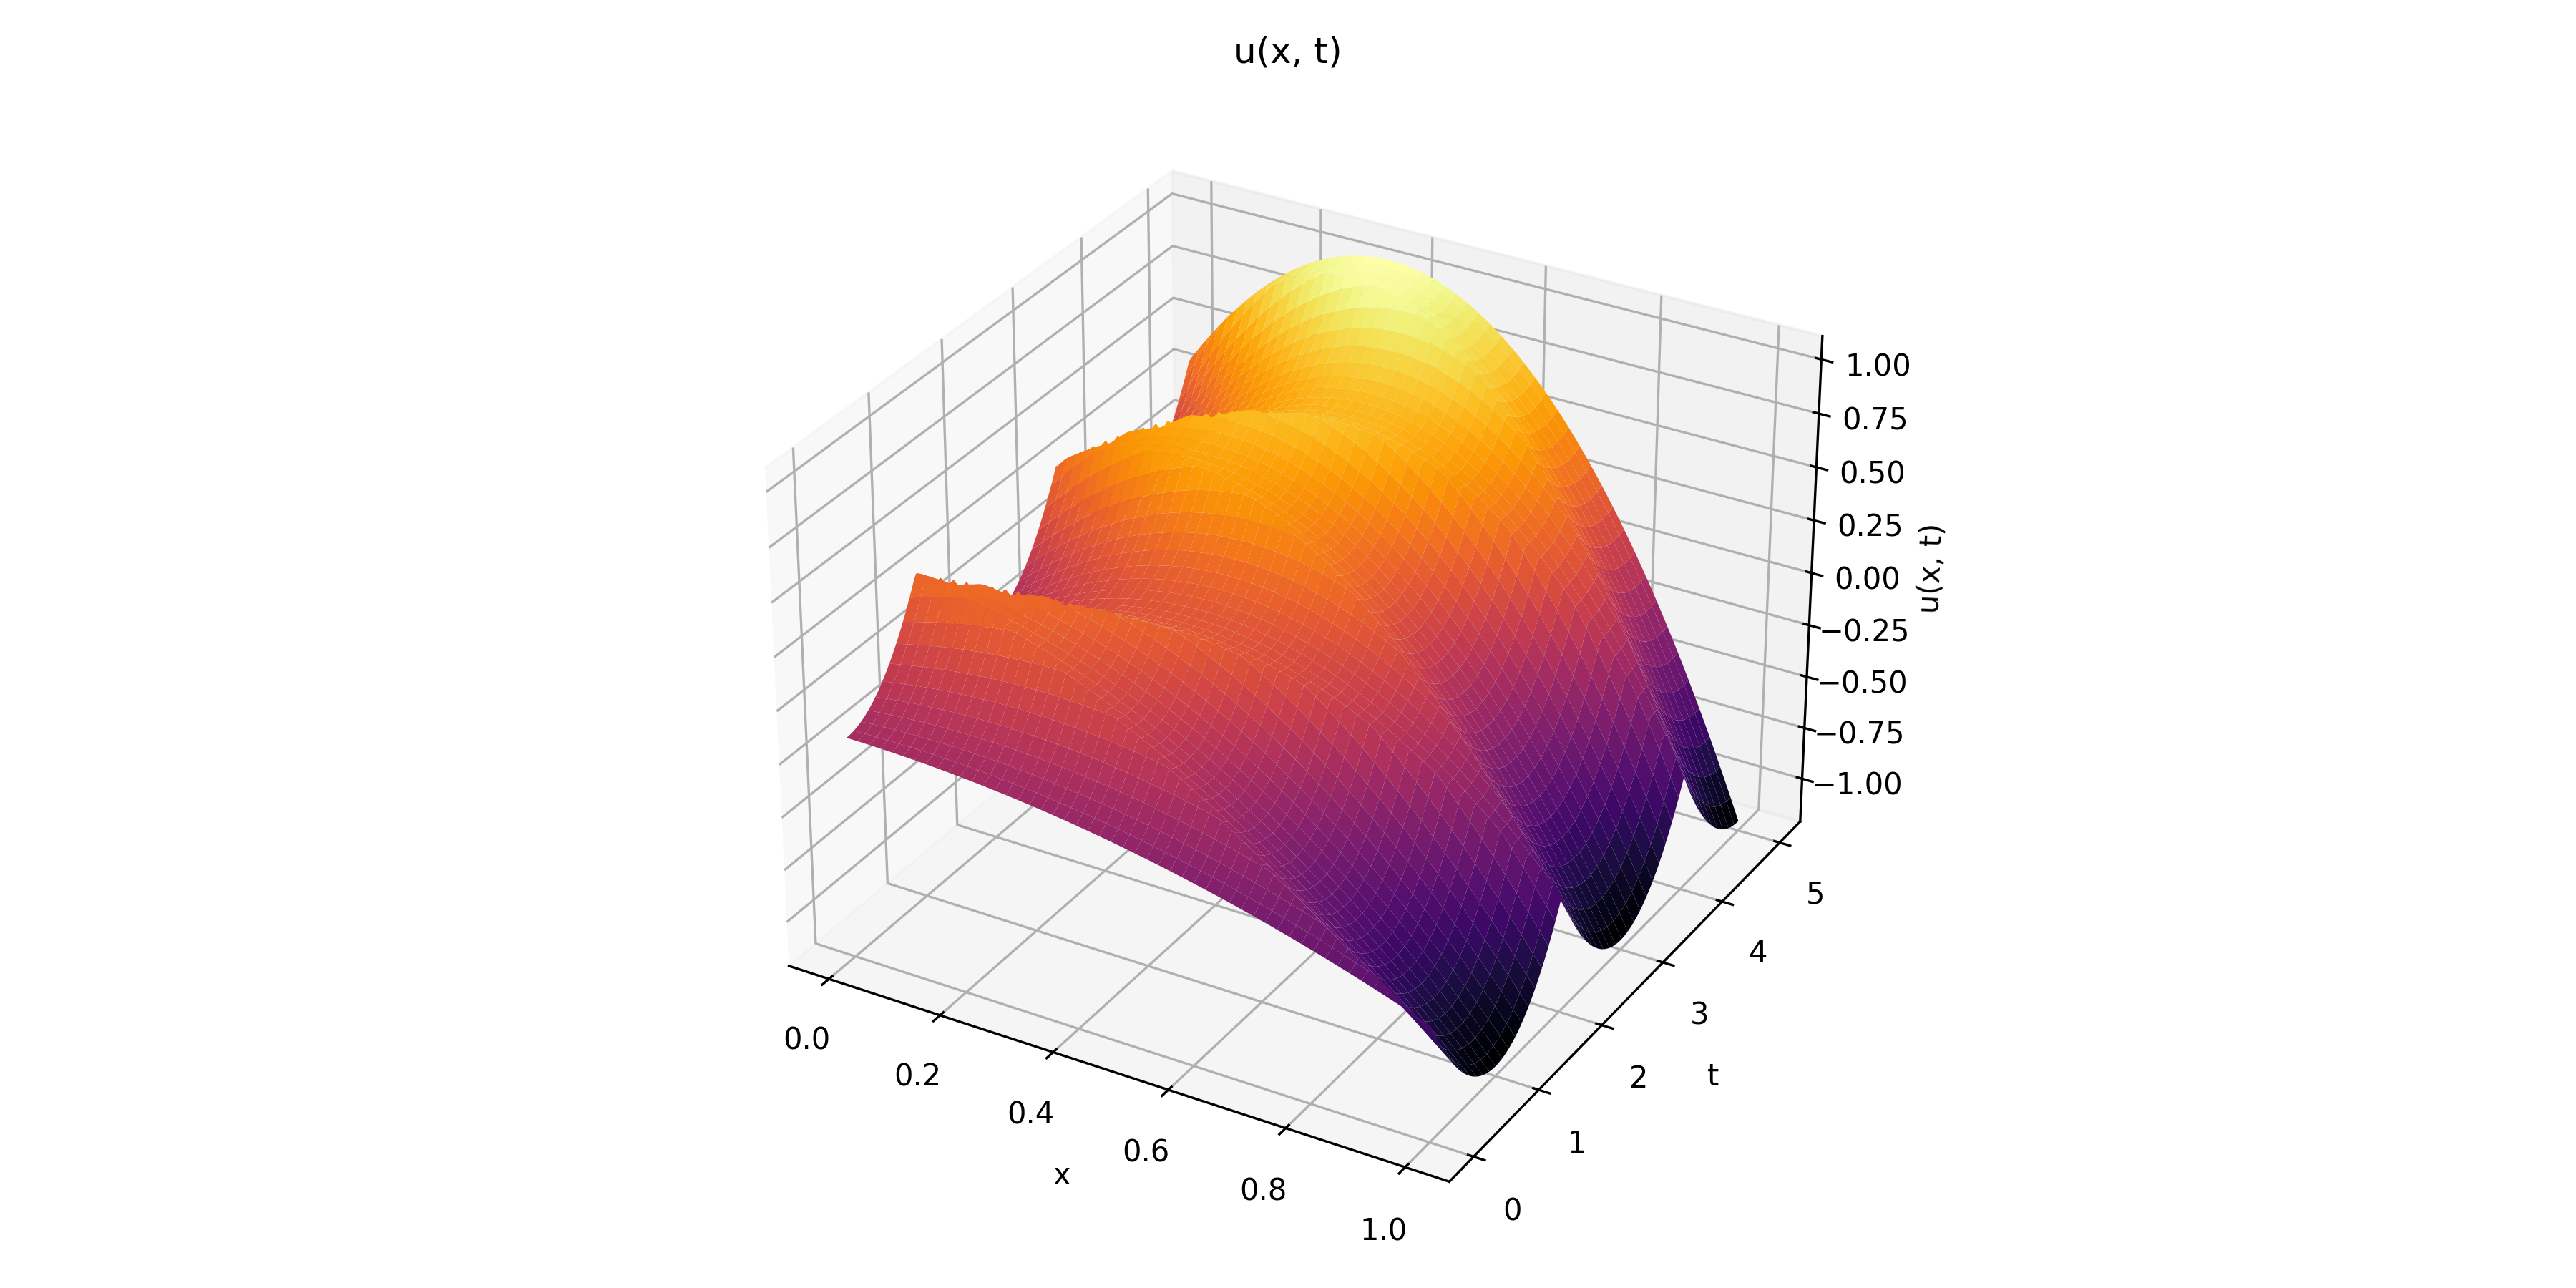
\includegraphics[width=0.8\textwidth]{../../graph3.png}
    \caption{График функции $u(x,t)$, построенный по приближённой сумме ряда}
\end{figure}

\textbf{Код проверки}
\begin{lstlisting}
eqn = D[u[x, t], {x, 2}] == f[x];
bc1 = u[0, t] == 2;
bc2 = Derivative[1, 0][u][0, t] == t;
bc3 = Derivative[1, 0][u][l, t] == -1;
ic1 = u[x, 0] == 0;
ic2 = Derivative[0, 1][u][x, 0] == 0;

solution = DSolve[{eqn, bc1, bc2, bc3, ic1, ic2}, u[x, t], {x, t}]

simplifiedSolution = Simplify[u[x, t] /. solution[[1]]]
\end{lstlisting}
\textbf{Результат проверки}
\begin{lstlisting}
    u[x_, t_, l_] := 
  Sum[(2 l Cos[Pi k])/((Pi k)^2) * Cos[(Pi k t)/l] * Cos[(Pi k x)/l], 
      {k, 1, Infinity}] - ((t + 1)/l) x^2 + t x
\end{lstlisting}

\end{document}
